\documentclass[12pt,letterpaper]{article}
\usepackage{graphicx,textcomp}
\usepackage{natbib}
\usepackage{setspace}
\usepackage{fullpage}
\usepackage{color}
\usepackage[reqno]{amsmath}
\usepackage{amsthm}
\usepackage{fancyvrb}
\usepackage{amssymb,enumerate}
\usepackage[all]{xy}
\usepackage{endnotes}
\usepackage{lscape}
\newtheorem{com}{Comment}
\usepackage{float}
\usepackage{hyperref}
\newtheorem{lem} {Lemma}
\newtheorem{prop}{Proposition}
\newtheorem{thm}{Theorem}
\newtheorem{defn}{Definition}
\newtheorem{cor}{Corollary}
\newtheorem{obs}{Observation}
\usepackage[compact]{titlesec}
\usepackage{dcolumn}
\usepackage{tikz}
\usetikzlibrary{arrows}
\usepackage{multirow}
\usepackage{xcolor}
\newcolumntype{.}{D{.}{.}{-1}}
\newcolumntype{d}[1]{D{.}{.}{#1}}
\definecolor{light-gray}{gray}{0.65}
\usepackage{url}
\usepackage{listings}
\usepackage{color}

\definecolor{codegreen}{rgb}{0,0.6,0}
\definecolor{codegray}{rgb}{0.5,0.5,0.5}
\definecolor{codepurple}{rgb}{0.58,0,0.82}
\definecolor{backcolour}{rgb}{0.95,0.95,0.92}

\lstdefinestyle{mystyle}{
	backgroundcolor=\color{backcolour},   
	commentstyle=\color{codegreen},
	keywordstyle=\color{magenta},
	numberstyle=\tiny\color{codegray},
	stringstyle=\color{codepurple},
	basicstyle=\footnotesize,
	breakatwhitespace=false,         
	breaklines=true,                 
	captionpos=b,                    
	keepspaces=true,                 
	numbers=left,                    
	numbersep=5pt,                  
	showspaces=false,                
	showstringspaces=false,
	showtabs=false,                  
	tabsize=2
}
\lstset{style=mystyle}
\newcommand{\Sref}[1]{Section~\ref{#1}}
\newtheorem{hyp}{Hypothesis}

\title{Problem Set 2}
\date{Due: October 15, 2021}
\author{Applied Stats/Quant Methods 1}

\begin{document}
	\maketitle
	\section*{Instructions}
\begin{itemize}
	\item Please show your work! You may lose points by simply writing in the answer. If the problem requires you to execute commands in \texttt{R}, please include the code you used to get your answers. Please also include the \texttt{.R} file that contains your code. If you are not sure if work needs to be shown for a particular problem, please ask.
	\item Your homework should be submitted electronically on GitHub in \texttt{.pdf} form.
	\item This problem set is due before class on Friday October 15, 2021. No late assignments will be accepted.
	\item Total available points for this homework is 100.
\end{itemize}

	
	\vspace{.5cm}
	\section*{Question 1 (40 points): Political Science}
		\vspace{.25cm}
	The following table was created using the data from a study run in a major Latin American city.\footnote{Fried, Lagunes, and Venkataramani (2010). ``Corruption and Inequality at the Crossroad: A Multimethod Study of Bribery and Discrimination in Latin America. \textit{Latin American Research Review}. 45 (1): 76-97.} As part of the experimental treatment in the study, one employee of the research team was chosen to make illegal left turns across traffic to draw the attention of the police officers on shift. Two employee drivers were upper class, two were lower class drivers, and the identity of the driver was randomly assigned per encounter. The researchers were interested in whether officers were more or less likely to solicit a bribe from drivers depending on their class (officers use phrases like, ``We can solve this the easy way'' to draw a bribe). The table below shows the resulting data.

\newpage
\begin{table}[h!]
	\centering
	\begin{tabular}{l | c c c }
		& Not Stopped & Bribe requested & Stopped/given warning \\
		\\[-1.8ex] 
		\hline \\[-1.8ex]
		Upper class & 14 & 6 & 7 \\
		Lower class & 7 & 7 & 1 \\
		\hline
	\end{tabular}
\end{table}

\begin{enumerate}
	
	\item [(a)]
	Calculate the $\chi^2$ test statistic by hand (even better if you can do "by hand" in \texttt{R}).\\
	\vspace{0.5cm}
	I did my chi square calculations by hand in R. First I created a matrix that would resemble the table provided in the task. 
	\lstinputlisting[language=R, firstline=13, lastline=18]{PS2_AC_Answer.R}
	After that I calculated the sums of all rows and columns in the table and I calculated my total value of all rows and columns.
	\lstinputlisting[language=R, firstline=24, lastline=30]{PS2_AC_Answer.R} 
	After that I calculated the expected frequencies of every observation in the table using formula: (total value of rows-grand total)/column total. 
	\lstinputlisting[language=R, firstline=34, lastline=39]{PS2_AC_Answer.R} 
	After that I calculated the quotient of expected and observed frequencies for each number in the table, following the formula: (observed frequencies-expected frequencies)squared/expected frequencies:
	\lstinputlisting[language=R, firstline=41, lastline=46]{PS2_AC_Answer.R}
	Sum of these quotients represents the chi square results which I got using the following formula:
	\lstinputlisting[language=R, firstline=48, lastline=48]{PS2_AC_Answer.R} 
	The final result of my chi square calculations is 21.75.
	
	\item [(b)]
	Now calculate the p-value from the test statistic you just created (in \texttt{R}).\footnote{Remember frequency should be $>$ 5 for all cells, but let's calculate the p-value here anyway.}  What do you conclude if $\alpha = .1$?\\
	To calculate my p value I first calculated my degrees of freedom by multiplying the number of rows and columns, both subtracted with 1 and following the standard formula for calculating the p value in R:
	\lstinputlisting[language=R, firstline=55, lastline=57]{PS2_AC_Answer.R}  
	As a way to check my results I ran a chisq.test function in R to compare the results, taking into account that there are cells in the table that have the frequency >5. 
	\lstinputlisting[language=R, firstline=61, lastline=62]{PS2_AC_Answer.R}
	Because the number of observations is not suited for calculations of the p value, there are inconsistencies. If calculated by hand, my p value = 1.893205e-05 and the p value got from the chi.square function is p = 0.1502. 
	To put the meaning of alpha value in context, I assume that:
	H0: class and bribe are independent variables.
	H1: class and bribe are not independent variables. 
	If alpha is the .1 then for my calculated p value I take that class and bribe are not independent variables, while function calculated p value is slightly bigger than alpha (I take that alpha is 0.10000), then it suggests how class and bribe are independent variables. 
	\vspace{1cm} 
	\item [(c)] Calculate the standardized residuals for each cell and put them in the table below.
	\vspace{1cm}
	
	\begin{table}[h]
		\centering
		\begin{tabular}{l | c c c }
			& Not Stopped & Bribe requested & Stopped/given warning \\
			\\[-1.8ex] 
			\hline \\[-1.8ex]
			Upper class  & 6.76 & 2.74 & 10.86 \\
			\\
			Lower class & 3.70 & 8.61  & -1.28  \\
			
		\end{tabular}
	\end{table}
	
	
	\vspace{7cm}
	\item [(d)] How might the standardized residuals help you interpret the results?  
	
	They are useful in helping to interpret chi-square tables by providing information about which cells contribute to a significant chi-square. If the standardized residual is beyond the range of ± 2, then that cell can be considered to be a major contributor, if it is > +2, or a very weak contributor, if it is beyond -2, to the overall chi-square value.
	A large standardized residual provides evidence against independence in that cell. When H0 is true, there is only about a 5\% chance that any particular standardized residual exceeds 2 in absolute value. From these residuals we see that the greatest contribution to the dependence of class and bribe provide the value of 10.86 for upper class and 8.61 for lower class, pointing that class and bribe are not independent.  
	
\end{enumerate}
\newpage

\section*{Question 2 (20 points): Economics}
Chattopadhyay and Duflo were interested in whether women promote different policies than men.\footnote{Chattopadhyay and Duflo. (2004). ``Women as Policy Makers: Evidence from a Randomized Policy Experiment in India. \textit{Econometrica}. 72 (5), 1409-1443.} Answering this question with observational data is pretty difficult due to potential confounding problems (e.g. the districts that choose female politicians are likely to systematically differ in other aspects too). Hence, they exploit a randomized policy experiment in India, where since the mid-1990s, $\frac{1}{3}$ of village council heads have been randomly reserved for women. A subset of the data from West Bengal can be found at the following link: \url{https://raw.githubusercontent.com/kosukeimai/qss/master/PREDICTION/women.csv}\\

\noindent Each observation in the data set represents a village and there are two villages associated with one GP (i.e. a level of government is called "GP"). Figure~\ref{fig:women_desc} below shows the names and descriptions of the variables in the dataset. The authors hypothesize that female politicians are more likely to support policies female voters want. Researchers found that more women complain about the quality of drinking water than men. You need to estimate the effect of the reservation policy on the number of new or repaired drinking water facilities in the villages.
\vspace{.5cm}
\begin{figure}[h!]
	\caption{\footnotesize{Names and description of variables from Chattopadhyay and Duflo (2004).}}
	\vspace{.5cm}
	\centering
	\label{fig:women_desc}
	%\includegraphics[width=1.1\textwidth]{../../../graphics/women_desc.png}
\end{figure}		

\newpage
\begin{enumerate}
	\item [(a)] State a null and alternative (two-tailed) hypothesis. 
	I constructed my hypothesis following the rule that H0 hypothesis indicates no relationship between the variables:
	
	H0: There is no effect of reservation policy on the number of new or repaired drinking water facilities.
	H1: There is an effect of reservation policy on the number of new or repaired drinking water facilities.
	
	\vspace{6cm}
	\item [(b)] Run a bivariate regression to test this hypothesis in \texttt{R} (include your code!).
	First I read the .csv file and for a pre-check I ran a linear model using the lm function in R: 
	\lstinputlisting[language=R, firstline=119, lastline=119]{PS2_AC_Answer.R}
	\lstinputlisting[language=R, firstline=133, lastline=137]{PS2_AC_Answer.R}
	
	After that I did my regression by hand:
	
	\lstinputlisting[language=R, firstline=141, lastline=174]{PS2_AC_Answer.R} 
	
	\vspace{1cm}
	\item [(c)] Interpret the coefficient estimate for reservation policy.
	
	In the model generated using the function my estimate beta coefficient is 9.25, which indicates that one more reserved space for women increases the number of new and repaired water facilities. My calculated beta is the same. Standard error in the model and by my calculations are the same (std. eror = 2.28) small levels of standard deviation or that means in the sample could differ from the estimated mean of the population for two standard deviations on average. My p value is the same as in the model calculated by function and suggests that there is statistical significance in the relationship between seats reserved for women and number of repaired water facilities (.01 < .05).
	
	 
\end{enumerate}

\newpage
	\section*{Question 3 (40 points): Biology}

There is a physiological cost of reproduction for fruit flies, such that it reduces the lifespan of female fruit flies.  Is there a similar cost to male fruit flies?  This dataset contains observations from five groups of 25 male fruit flies. The experiment tests if increased reproduction reduces longevity for male fruit flies. The five groups are: males forced to live alone, males assigned to live with one or eight newly pregnant females (non-receptive females), and males assigned to live with one or eight virgin females (interested females). The name of the data set is \texttt{fruitfly.csv}.\footnote{Partridge and Farquhar (1981).``Sexual Activity and the Lifespan of Male Fruitflies''. \textit{Nature}. 294, 580-581.}
	\vspace{1cm}

\begin{tabular}{r|l}
	\texttt{No} & serial number (1-25) within each group of 25\\
	\texttt{type} & Type of experimental assignment \\
	& \hspace{0.1in} $1=$ no females  \\
	& \hspace{0.1in} $2=$ 1 newly pregnant female \\
	& \hspace{0.1in} $3=$ 8 newly pregnant females\\
	& \hspace{0.1in} $4=$ 1 virgin female\\
	& \hspace{0.1in} $5=$ 8 virgin females\\
	\texttt{lifespan} & lifespan (days)\\
	\texttt{thorax} & length of thorax (mm)\\
	\texttt{sleep} & percentage of each day spent sleeping\\
\end{tabular}
	\vspace{1cm}
\begin{enumerate}
	
	\item
	Import the data set and obtain summary statistiscs and examine the distribution of the overall lifespan of the fruitflies.  
	I inspected my dataset using the summary function in R:
	\lstinputlisting[language=R, firstline=182, lastline=186]{PS2_AC_Answer.R}
	From the summary, I read that the min. longevity of a fruit fly is 16 and max. 97. (not sure about the units, so I report numbers only). Mean is 57.44. 
\vspace{1cm}
	\item
	Plot \texttt{lifespan} vs \texttt{thorax}. Does it look like there is a linear relationship? Provide the plot. What is the correlation coefficient between these two variables?
	
	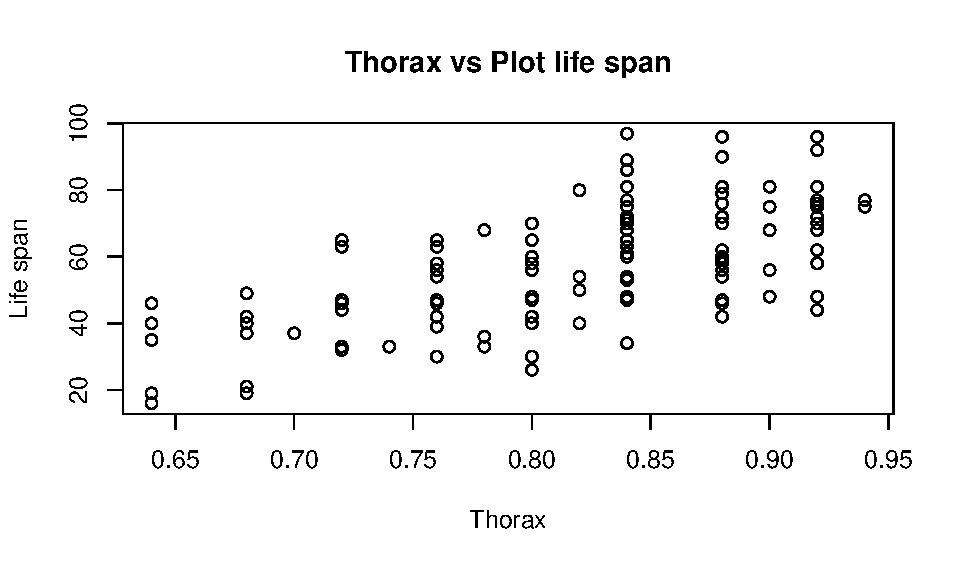
\includegraphics{Rplot01}
	
	I rendered the graph using the following formula:
	\lstinputlisting[language=R, firstline=190, lastline=193]{PS2_AC_Answer.R}
	
	My correlation result is 0.63 which indicates medium strong level of association.
	
	I used the following formula for the correlation:
	\lstinputlisting[language=R, firstline=195, lastline=196]{PS2_AC_Answer.R}
	
	\item
	Regress \texttt{lifespan} on \texttt{thorax}.  Interpret the slope of the fitted model.
			\vspace{1cm}
			
	I regressed the results and rendered the slope using the following formula: 
	\lstinputlisting[language=R, firstline=201, lastline=204]{PS2_AC_Answer.R}
	
	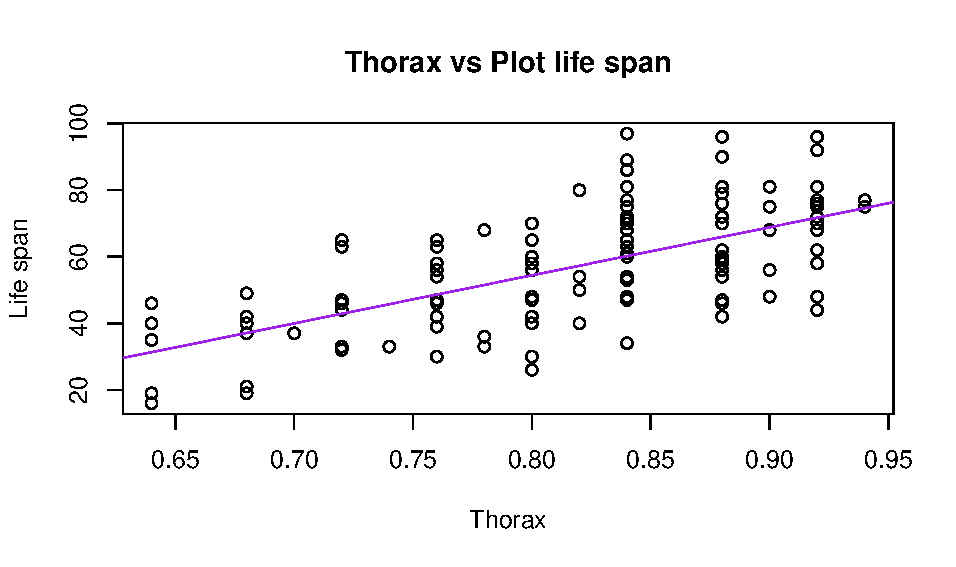
\includegraphics{Rplot02}
	
	The slope of the fitted model indicates the linear relationship in the data and that the size of thorax is positively associated with the lifespan of a fruit fly. 
	
	\item
	Test for a significant linear relationship between  \texttt{lifespan} and \texttt{thorax}. Provide and interpret your results of your test. 
	
	I tested the significance of linear relationship using the chi square test. 
	\lstinputlisting[language=R, firstline=209, lastline=210]{PS2_AC_Answer.R}
	I got that the association between the size of thorax and the lifespan is statistically significant the p value of .05. And the association according to the chi square is strong (=642).
	
\newpage
	\item
	
	Provide the 90\% confidence interval for the slope of the fitted model.
	
			\vspace{.5cm}
	\begin{itemize}
		\item
		Use the formula of confidence interval.		\vspace{.5cm}
		\item
		Use the function  \texttt{confint()}  in \texttt{R} .
	\end{itemize}
			\vspace{1cm}
	My work gets really sloppy at this point and I am not sure why my results are not proper at this point. As per task, I calculated the CI by hand:
	
	\lstinputlisting[language=R, firstline=216, lastline=231]{PS2_AC_Answer.R}
	
	I got as my lower CI = -1.38e-11 and as my upper CI = 0.0056136. Which I am not sure how to interpret. Using formula confint I did not manage to get proper results and my calculations rendered NA as a result. I used the following formula:
	
	\lstinputlisting[language=R, firstline=235, lastline=235]{PS2_AC_Answer.R}
	
	\item Use the \texttt{predict()} function in \texttt{R} to (1) predict an individual fruitfly's lifespan when \texttt{thorax}=0.8 and (2) the average \texttt{lifespan} of fruitflies when \texttt{thorax}=0.8 by the fitted model. This requires that you compute prediction and confidence intervals. What are the expected values of lifespan? What are the prediction and confidence intervals around the expected values? 
	
			\vspace{1cm}
		I tried doing this one and following one. You can see some of mu R code, but I started getting the error message which I did not know how to amend. The message says that the data in my formula is the wrong, i.e. it is an lm object which I tried turning into data frame or list, but I was not successful. 
	\item	For a sequence of \texttt{thorax} values, draw a plot with their fitted values for \texttt{lifespan}, as well as the prediction intervals and confidence intervals.



\end{enumerate}
\end{document}
